\begin{figure*}[t]
  \centering
  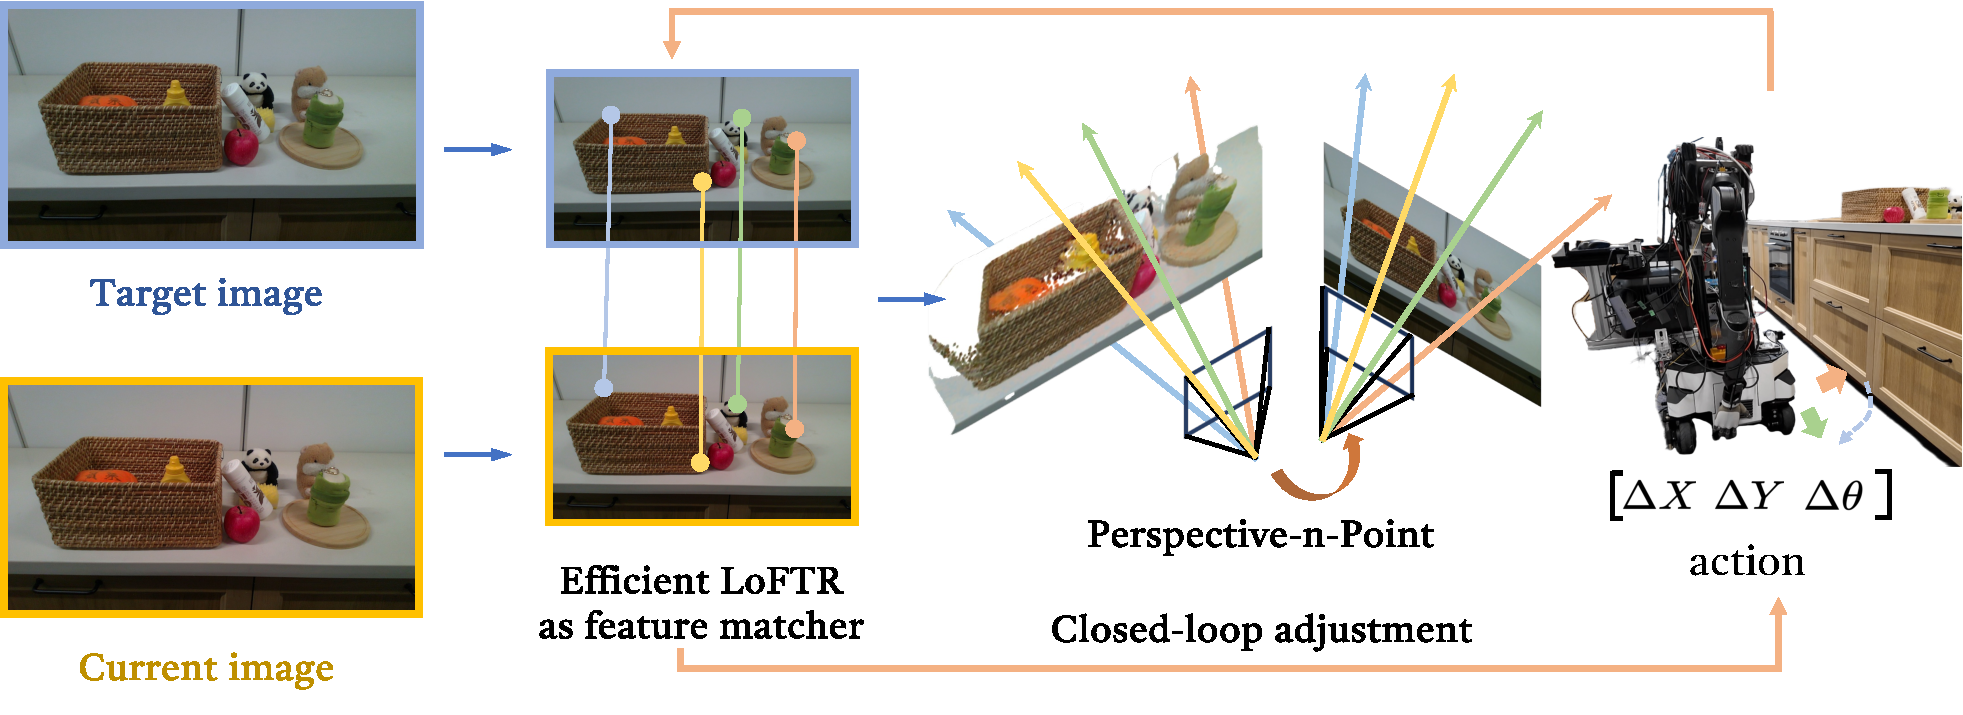
\includegraphics[width=1.0\linewidth]{figures/realtime-pnp_pic.pdf}
  \vspace{-15pt}
  \caption{ \textbf{The pipeline of closed-loop PnP localization.} We first employ the Efficient LoFTR  to extract dense visual correspondence, followed by estimating the transformation between the current frame and the goal location via solving the PnP problem. Subsequently, we use PID controller to execute the action. This entire process is executed in a closed-loop manner and continues iteratively until the spatial discrepancy between the robot's current pose and the goal falls below a predefined threshold.}
  \label{fig:realtime-pnp}
\end{figure*}